\INEchaptercarta{Niñez que labora y su escolaridad}{}



\cajita{Tasa de trabajo infantil}{}{Tasa de la población menor a 14 años que realiza actividades económicas}{República de Guatemala, serie histórica, en porcentaje}{\ \\[0mm]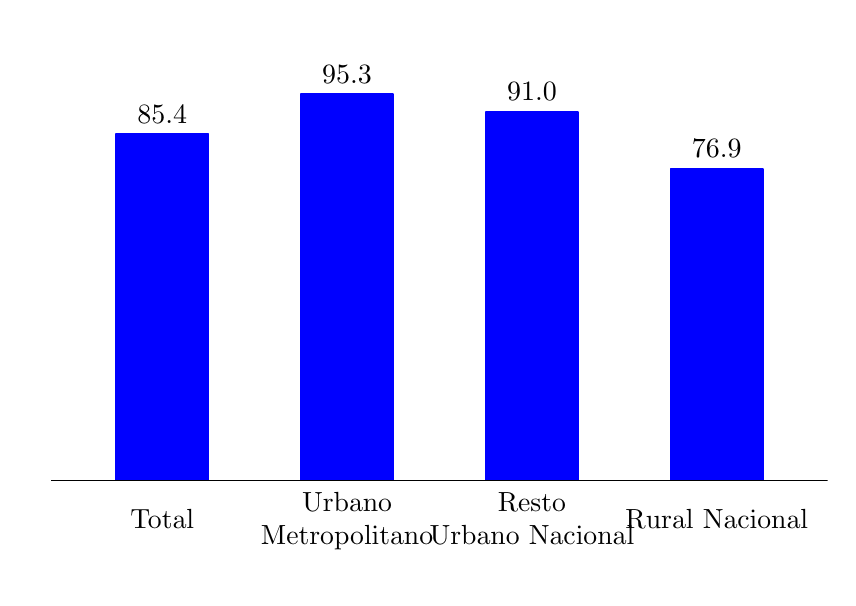
\begin{tikzpicture}[x=1pt,y=1pt]  % Created by tikzDevice version 0.9 on 2015-12-11 10:47:36
% !TEX encoding = UTF-8 Unicode
\definecolor{fillColor}{RGB}{255,255,255}
\path[use as bounding box,fill=fillColor,fill opacity=0.00] (0,0) rectangle (289.08,198.74);
\begin{scope}
\path[clip] (  0.00,  0.00) rectangle (289.08,198.74);

\path[] (  0.00,  0.00) rectangle (289.08,198.74);
\end{scope}
\begin{scope}
\path[clip] (  0.00,  0.00) rectangle (289.08,198.74);

\path[] (  8.54, 28.23) rectangle (289.08,181.67);

\path[] ( 48.61, 28.23) --
	( 48.61,181.67);

\path[] (115.41, 28.23) --
	(115.41,181.67);

\path[] (182.21, 28.23) --
	(182.21,181.67);

\path[] (249.00, 28.23) --
	(249.00,181.67);
\definecolor{drawColor}{RGB}{0,0,255}
\definecolor{fillColor}{RGB}{0,0,255}

\path[draw=drawColor,line width= 0.6pt,line join=round,fill=fillColor] ( 31.91, 35.21) rectangle ( 65.31,160.24);

\path[draw=drawColor,line width= 0.6pt,line join=round,fill=fillColor] ( 98.71, 35.21) rectangle (132.11,174.70);

\path[draw=drawColor,line width= 0.6pt,line join=round,fill=fillColor] (165.51, 35.21) rectangle (198.91,168.34);

\path[draw=drawColor,line width= 0.6pt,line join=round,fill=fillColor] (232.30, 35.21) rectangle (265.70,147.71);
\definecolor{drawColor}{RGB}{0,0,0}

\path[draw=drawColor,line width= 0.1pt,line join=round] (  8.54, 35.21) -- (289.08, 35.21);

\node[text=drawColor,anchor=base,inner sep=0pt, outer sep=0pt, scale=  1.01] at ( 48.61,164.19) {85.4};

\node[text=drawColor,anchor=base,inner sep=0pt, outer sep=0pt, scale=  1.01] at (115.41,178.65) {95.3};

\node[text=drawColor,anchor=base,inner sep=0pt, outer sep=0pt, scale=  1.01] at (182.21,172.29) {91.0};

\node[text=drawColor,anchor=base,inner sep=0pt, outer sep=0pt, scale=  1.01] at (249.00,151.66) {76.9};

\path[] (  8.54, 28.23) rectangle (289.08,181.67);
\end{scope}
\begin{scope}
\path[clip] (  0.00,  0.00) rectangle (289.08,198.74);

\path[] (  8.54, 28.23) --
	(  8.54,181.67);
\end{scope}
\begin{scope}
\path[clip] (  0.00,  0.00) rectangle (289.08,198.74);

\path[] (  8.54, 28.23) --
	(289.08, 28.23);
\end{scope}
\begin{scope}
\path[clip] (  0.00,  0.00) rectangle (289.08,198.74);

\path[] ( 48.61, 23.96) --
	( 48.61, 28.23);

\path[] (115.41, 23.96) --
	(115.41, 28.23);

\path[] (182.21, 23.96) --
	(182.21, 28.23);

\path[] (249.00, 23.96) --
	(249.00, 28.23);
\end{scope}
\begin{scope}
\path[clip] (  0.00,  0.00) rectangle (289.08,198.74);
\definecolor{drawColor}{RGB}{0,0,0}

\node[text=drawColor,anchor=base,inner sep=0pt, outer sep=0pt, scale=  1.00] at ( 48.61, 17.92) {Total};

\node[text=drawColor,anchor=base,inner sep=0pt, outer sep=0pt, scale=  1.00] at (115.41, 23.86) {Urbano };

\node[text=drawColor,anchor=base,inner sep=0pt, outer sep=0pt, scale=  1.00] at (115.41, 11.98) { Metropolitano};

\node[text=drawColor,anchor=base,inner sep=0pt, outer sep=0pt, scale=  1.00] at (182.21, 23.86) {Resto };

\node[text=drawColor,anchor=base,inner sep=0pt, outer sep=0pt, scale=  1.00] at (182.21, 11.98) { Urbano Nacional};

\node[text=drawColor,anchor=base,inner sep=0pt, outer sep=0pt, scale=  1.00] at (249.00, 17.92) {Rural Nacional};
\end{scope}
  \end{tikzpicture} }{Instituto Nacional de Estadística, con datos de ENEI II-2014}



\cajita{Tasa de trabajo infantil por sexo}{}{Tasa de la población menor a 14 años que realiza actividades económicas según sexo}{República de Guatemala, año 2014, en porcentaje}{\ \\[0mm]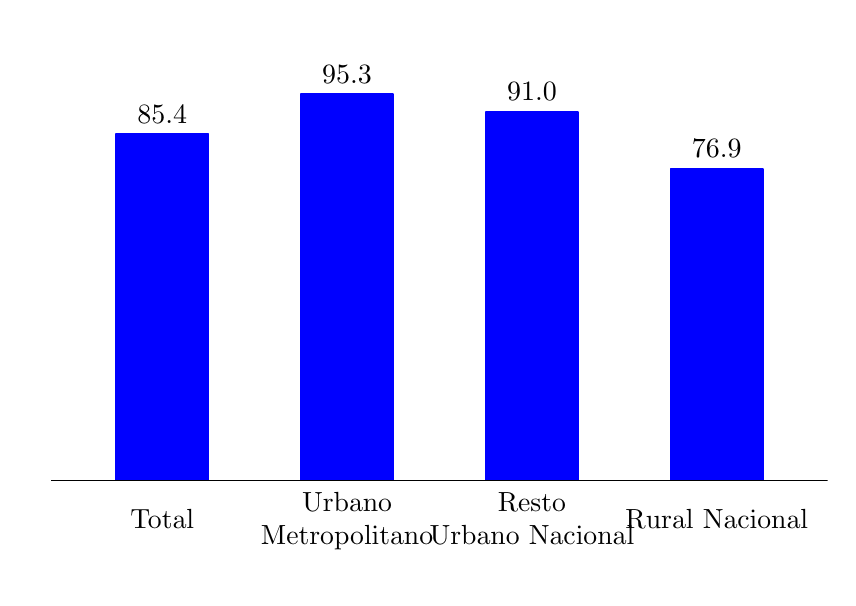
\begin{tikzpicture}[x=1pt,y=1pt]  % Created by tikzDevice version 0.9 on 2015-12-11 10:47:36
% !TEX encoding = UTF-8 Unicode
\definecolor{fillColor}{RGB}{255,255,255}
\path[use as bounding box,fill=fillColor,fill opacity=0.00] (0,0) rectangle (289.08,198.74);
\begin{scope}
\path[clip] (  0.00,  0.00) rectangle (289.08,198.74);

\path[] (  0.00,  0.00) rectangle (289.08,198.74);
\end{scope}
\begin{scope}
\path[clip] (  0.00,  0.00) rectangle (289.08,198.74);

\path[] (  8.54, 28.23) rectangle (289.08,181.67);

\path[] ( 48.61, 28.23) --
	( 48.61,181.67);

\path[] (115.41, 28.23) --
	(115.41,181.67);

\path[] (182.21, 28.23) --
	(182.21,181.67);

\path[] (249.00, 28.23) --
	(249.00,181.67);
\definecolor{drawColor}{RGB}{0,0,255}
\definecolor{fillColor}{RGB}{0,0,255}

\path[draw=drawColor,line width= 0.6pt,line join=round,fill=fillColor] ( 31.91, 35.21) rectangle ( 65.31,160.24);

\path[draw=drawColor,line width= 0.6pt,line join=round,fill=fillColor] ( 98.71, 35.21) rectangle (132.11,174.70);

\path[draw=drawColor,line width= 0.6pt,line join=round,fill=fillColor] (165.51, 35.21) rectangle (198.91,168.34);

\path[draw=drawColor,line width= 0.6pt,line join=round,fill=fillColor] (232.30, 35.21) rectangle (265.70,147.71);
\definecolor{drawColor}{RGB}{0,0,0}

\path[draw=drawColor,line width= 0.1pt,line join=round] (  8.54, 35.21) -- (289.08, 35.21);

\node[text=drawColor,anchor=base,inner sep=0pt, outer sep=0pt, scale=  1.01] at ( 48.61,164.19) {85.4};

\node[text=drawColor,anchor=base,inner sep=0pt, outer sep=0pt, scale=  1.01] at (115.41,178.65) {95.3};

\node[text=drawColor,anchor=base,inner sep=0pt, outer sep=0pt, scale=  1.01] at (182.21,172.29) {91.0};

\node[text=drawColor,anchor=base,inner sep=0pt, outer sep=0pt, scale=  1.01] at (249.00,151.66) {76.9};

\path[] (  8.54, 28.23) rectangle (289.08,181.67);
\end{scope}
\begin{scope}
\path[clip] (  0.00,  0.00) rectangle (289.08,198.74);

\path[] (  8.54, 28.23) --
	(  8.54,181.67);
\end{scope}
\begin{scope}
\path[clip] (  0.00,  0.00) rectangle (289.08,198.74);

\path[] (  8.54, 28.23) --
	(289.08, 28.23);
\end{scope}
\begin{scope}
\path[clip] (  0.00,  0.00) rectangle (289.08,198.74);

\path[] ( 48.61, 23.96) --
	( 48.61, 28.23);

\path[] (115.41, 23.96) --
	(115.41, 28.23);

\path[] (182.21, 23.96) --
	(182.21, 28.23);

\path[] (249.00, 23.96) --
	(249.00, 28.23);
\end{scope}
\begin{scope}
\path[clip] (  0.00,  0.00) rectangle (289.08,198.74);
\definecolor{drawColor}{RGB}{0,0,0}

\node[text=drawColor,anchor=base,inner sep=0pt, outer sep=0pt, scale=  1.00] at ( 48.61, 17.92) {Total};

\node[text=drawColor,anchor=base,inner sep=0pt, outer sep=0pt, scale=  1.00] at (115.41, 23.86) {Urbano };

\node[text=drawColor,anchor=base,inner sep=0pt, outer sep=0pt, scale=  1.00] at (115.41, 11.98) { Metropolitano};

\node[text=drawColor,anchor=base,inner sep=0pt, outer sep=0pt, scale=  1.00] at (182.21, 23.86) {Resto };

\node[text=drawColor,anchor=base,inner sep=0pt, outer sep=0pt, scale=  1.00] at (182.21, 11.98) { Urbano Nacional};

\node[text=drawColor,anchor=base,inner sep=0pt, outer sep=0pt, scale=  1.00] at (249.00, 17.92) {Rural Nacional};
\end{scope}
  \end{tikzpicture} }{Instituto Nacional de Estadística, con datos de ENEI II-2014}


\cajita{Trabajo infantil y anpea por dominio de estudio}{}{Proporción de la población menor a 14 años que realiza actividades económicas, por dominio de estudio}{República de Guatemala, año 2014, en porcentaje}{\ \\[0mm]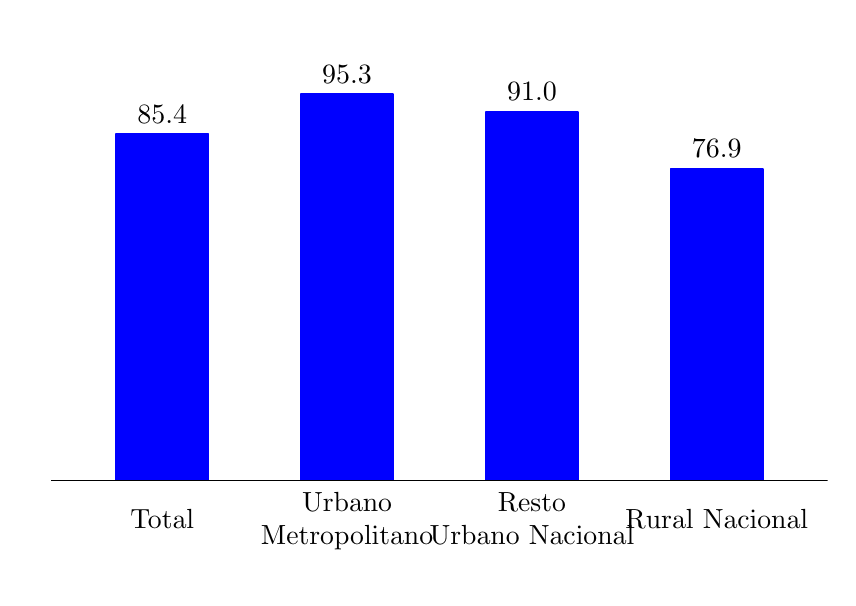
\begin{tikzpicture}[x=1pt,y=1pt]  % Created by tikzDevice version 0.9 on 2015-12-11 10:47:36
% !TEX encoding = UTF-8 Unicode
\definecolor{fillColor}{RGB}{255,255,255}
\path[use as bounding box,fill=fillColor,fill opacity=0.00] (0,0) rectangle (289.08,198.74);
\begin{scope}
\path[clip] (  0.00,  0.00) rectangle (289.08,198.74);

\path[] (  0.00,  0.00) rectangle (289.08,198.74);
\end{scope}
\begin{scope}
\path[clip] (  0.00,  0.00) rectangle (289.08,198.74);

\path[] (  8.54, 28.23) rectangle (289.08,181.67);

\path[] ( 48.61, 28.23) --
	( 48.61,181.67);

\path[] (115.41, 28.23) --
	(115.41,181.67);

\path[] (182.21, 28.23) --
	(182.21,181.67);

\path[] (249.00, 28.23) --
	(249.00,181.67);
\definecolor{drawColor}{RGB}{0,0,255}
\definecolor{fillColor}{RGB}{0,0,255}

\path[draw=drawColor,line width= 0.6pt,line join=round,fill=fillColor] ( 31.91, 35.21) rectangle ( 65.31,160.24);

\path[draw=drawColor,line width= 0.6pt,line join=round,fill=fillColor] ( 98.71, 35.21) rectangle (132.11,174.70);

\path[draw=drawColor,line width= 0.6pt,line join=round,fill=fillColor] (165.51, 35.21) rectangle (198.91,168.34);

\path[draw=drawColor,line width= 0.6pt,line join=round,fill=fillColor] (232.30, 35.21) rectangle (265.70,147.71);
\definecolor{drawColor}{RGB}{0,0,0}

\path[draw=drawColor,line width= 0.1pt,line join=round] (  8.54, 35.21) -- (289.08, 35.21);

\node[text=drawColor,anchor=base,inner sep=0pt, outer sep=0pt, scale=  1.01] at ( 48.61,164.19) {85.4};

\node[text=drawColor,anchor=base,inner sep=0pt, outer sep=0pt, scale=  1.01] at (115.41,178.65) {95.3};

\node[text=drawColor,anchor=base,inner sep=0pt, outer sep=0pt, scale=  1.01] at (182.21,172.29) {91.0};

\node[text=drawColor,anchor=base,inner sep=0pt, outer sep=0pt, scale=  1.01] at (249.00,151.66) {76.9};

\path[] (  8.54, 28.23) rectangle (289.08,181.67);
\end{scope}
\begin{scope}
\path[clip] (  0.00,  0.00) rectangle (289.08,198.74);

\path[] (  8.54, 28.23) --
	(  8.54,181.67);
\end{scope}
\begin{scope}
\path[clip] (  0.00,  0.00) rectangle (289.08,198.74);

\path[] (  8.54, 28.23) --
	(289.08, 28.23);
\end{scope}
\begin{scope}
\path[clip] (  0.00,  0.00) rectangle (289.08,198.74);

\path[] ( 48.61, 23.96) --
	( 48.61, 28.23);

\path[] (115.41, 23.96) --
	(115.41, 28.23);

\path[] (182.21, 23.96) --
	(182.21, 28.23);

\path[] (249.00, 23.96) --
	(249.00, 28.23);
\end{scope}
\begin{scope}
\path[clip] (  0.00,  0.00) rectangle (289.08,198.74);
\definecolor{drawColor}{RGB}{0,0,0}

\node[text=drawColor,anchor=base,inner sep=0pt, outer sep=0pt, scale=  1.00] at ( 48.61, 17.92) {Total};

\node[text=drawColor,anchor=base,inner sep=0pt, outer sep=0pt, scale=  1.00] at (115.41, 23.86) {Urbano };

\node[text=drawColor,anchor=base,inner sep=0pt, outer sep=0pt, scale=  1.00] at (115.41, 11.98) { Metropolitano};

\node[text=drawColor,anchor=base,inner sep=0pt, outer sep=0pt, scale=  1.00] at (182.21, 23.86) {Resto };

\node[text=drawColor,anchor=base,inner sep=0pt, outer sep=0pt, scale=  1.00] at (182.21, 11.98) { Urbano Nacional};

\node[text=drawColor,anchor=base,inner sep=0pt, outer sep=0pt, scale=  1.00] at (249.00, 17.92) {Rural Nacional};
\end{scope}
  \end{tikzpicture} }{Instituto Nacional de Estadística, con datos de ENEI II-2014}


\cajita{Trabajo infantil y escolaridad}{}{Proporción de la población menor a 14 años que realiza actividades económicas, por nivel de escolaridad}{República de Guatemala, año 2014, en porcentaje}{\ \\[0mm]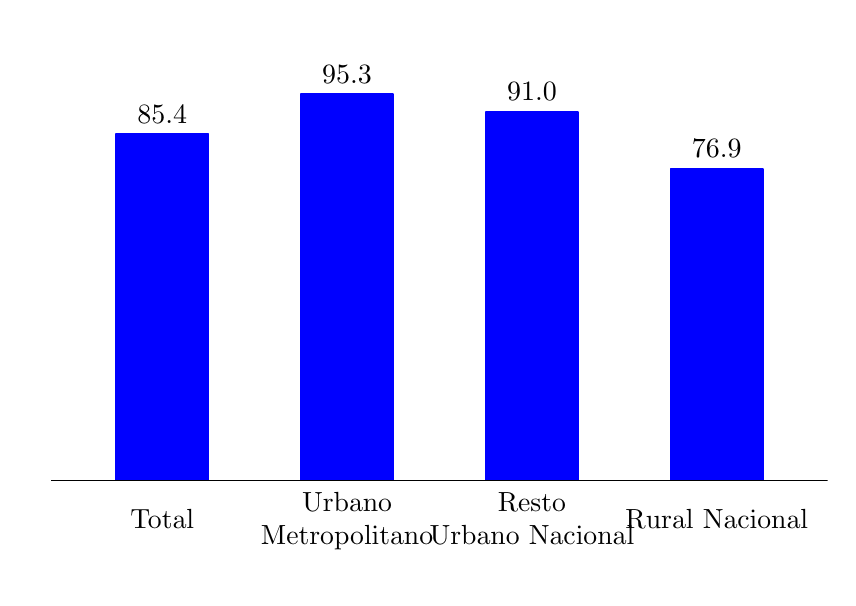
\begin{tikzpicture}[x=1pt,y=1pt]  % Created by tikzDevice version 0.9 on 2015-12-11 10:47:36
% !TEX encoding = UTF-8 Unicode
\definecolor{fillColor}{RGB}{255,255,255}
\path[use as bounding box,fill=fillColor,fill opacity=0.00] (0,0) rectangle (289.08,198.74);
\begin{scope}
\path[clip] (  0.00,  0.00) rectangle (289.08,198.74);

\path[] (  0.00,  0.00) rectangle (289.08,198.74);
\end{scope}
\begin{scope}
\path[clip] (  0.00,  0.00) rectangle (289.08,198.74);

\path[] (  8.54, 28.23) rectangle (289.08,181.67);

\path[] ( 48.61, 28.23) --
	( 48.61,181.67);

\path[] (115.41, 28.23) --
	(115.41,181.67);

\path[] (182.21, 28.23) --
	(182.21,181.67);

\path[] (249.00, 28.23) --
	(249.00,181.67);
\definecolor{drawColor}{RGB}{0,0,255}
\definecolor{fillColor}{RGB}{0,0,255}

\path[draw=drawColor,line width= 0.6pt,line join=round,fill=fillColor] ( 31.91, 35.21) rectangle ( 65.31,160.24);

\path[draw=drawColor,line width= 0.6pt,line join=round,fill=fillColor] ( 98.71, 35.21) rectangle (132.11,174.70);

\path[draw=drawColor,line width= 0.6pt,line join=round,fill=fillColor] (165.51, 35.21) rectangle (198.91,168.34);

\path[draw=drawColor,line width= 0.6pt,line join=round,fill=fillColor] (232.30, 35.21) rectangle (265.70,147.71);
\definecolor{drawColor}{RGB}{0,0,0}

\path[draw=drawColor,line width= 0.1pt,line join=round] (  8.54, 35.21) -- (289.08, 35.21);

\node[text=drawColor,anchor=base,inner sep=0pt, outer sep=0pt, scale=  1.01] at ( 48.61,164.19) {85.4};

\node[text=drawColor,anchor=base,inner sep=0pt, outer sep=0pt, scale=  1.01] at (115.41,178.65) {95.3};

\node[text=drawColor,anchor=base,inner sep=0pt, outer sep=0pt, scale=  1.01] at (182.21,172.29) {91.0};

\node[text=drawColor,anchor=base,inner sep=0pt, outer sep=0pt, scale=  1.01] at (249.00,151.66) {76.9};

\path[] (  8.54, 28.23) rectangle (289.08,181.67);
\end{scope}
\begin{scope}
\path[clip] (  0.00,  0.00) rectangle (289.08,198.74);

\path[] (  8.54, 28.23) --
	(  8.54,181.67);
\end{scope}
\begin{scope}
\path[clip] (  0.00,  0.00) rectangle (289.08,198.74);

\path[] (  8.54, 28.23) --
	(289.08, 28.23);
\end{scope}
\begin{scope}
\path[clip] (  0.00,  0.00) rectangle (289.08,198.74);

\path[] ( 48.61, 23.96) --
	( 48.61, 28.23);

\path[] (115.41, 23.96) --
	(115.41, 28.23);

\path[] (182.21, 23.96) --
	(182.21, 28.23);

\path[] (249.00, 23.96) --
	(249.00, 28.23);
\end{scope}
\begin{scope}
\path[clip] (  0.00,  0.00) rectangle (289.08,198.74);
\definecolor{drawColor}{RGB}{0,0,0}

\node[text=drawColor,anchor=base,inner sep=0pt, outer sep=0pt, scale=  1.00] at ( 48.61, 17.92) {Total};

\node[text=drawColor,anchor=base,inner sep=0pt, outer sep=0pt, scale=  1.00] at (115.41, 23.86) {Urbano };

\node[text=drawColor,anchor=base,inner sep=0pt, outer sep=0pt, scale=  1.00] at (115.41, 11.98) { Metropolitano};

\node[text=drawColor,anchor=base,inner sep=0pt, outer sep=0pt, scale=  1.00] at (182.21, 23.86) {Resto };

\node[text=drawColor,anchor=base,inner sep=0pt, outer sep=0pt, scale=  1.00] at (182.21, 11.98) { Urbano Nacional};

\node[text=drawColor,anchor=base,inner sep=0pt, outer sep=0pt, scale=  1.00] at (249.00, 17.92) {Rural Nacional};
\end{scope}
  \end{tikzpicture} }{Instituto Nacional de Estadística, con datos de ENEI II-2014}


\cajita{Trabajo infantil, escolaridad y sexo}{}{Proporción de la población menor a 14 años que realiza actividades económicas, por nivel de escolaridad y sexo}{República de Guatemala, año 2014, en porcentaje}{\ \\[0mm]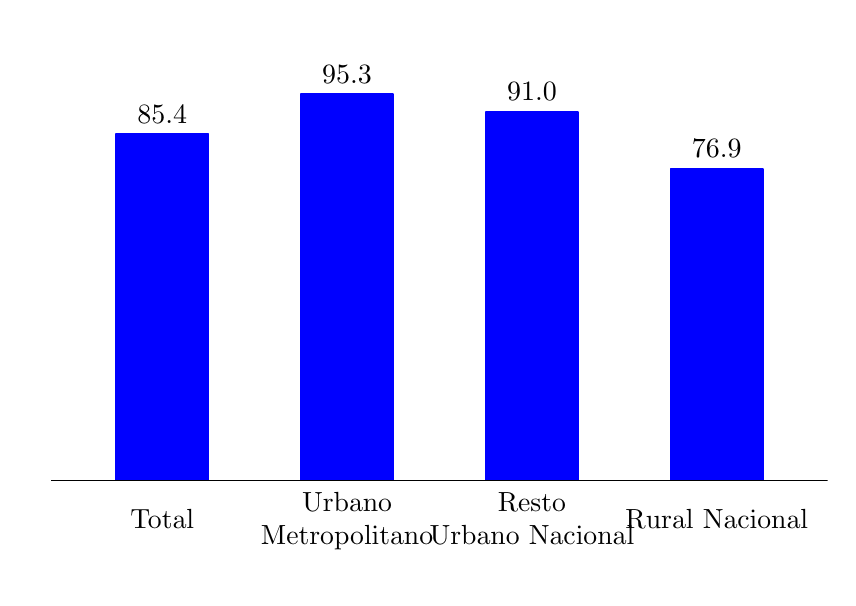
\begin{tikzpicture}[x=1pt,y=1pt]  % Created by tikzDevice version 0.9 on 2015-12-11 10:47:36
% !TEX encoding = UTF-8 Unicode
\definecolor{fillColor}{RGB}{255,255,255}
\path[use as bounding box,fill=fillColor,fill opacity=0.00] (0,0) rectangle (289.08,198.74);
\begin{scope}
\path[clip] (  0.00,  0.00) rectangle (289.08,198.74);

\path[] (  0.00,  0.00) rectangle (289.08,198.74);
\end{scope}
\begin{scope}
\path[clip] (  0.00,  0.00) rectangle (289.08,198.74);

\path[] (  8.54, 28.23) rectangle (289.08,181.67);

\path[] ( 48.61, 28.23) --
	( 48.61,181.67);

\path[] (115.41, 28.23) --
	(115.41,181.67);

\path[] (182.21, 28.23) --
	(182.21,181.67);

\path[] (249.00, 28.23) --
	(249.00,181.67);
\definecolor{drawColor}{RGB}{0,0,255}
\definecolor{fillColor}{RGB}{0,0,255}

\path[draw=drawColor,line width= 0.6pt,line join=round,fill=fillColor] ( 31.91, 35.21) rectangle ( 65.31,160.24);

\path[draw=drawColor,line width= 0.6pt,line join=round,fill=fillColor] ( 98.71, 35.21) rectangle (132.11,174.70);

\path[draw=drawColor,line width= 0.6pt,line join=round,fill=fillColor] (165.51, 35.21) rectangle (198.91,168.34);

\path[draw=drawColor,line width= 0.6pt,line join=round,fill=fillColor] (232.30, 35.21) rectangle (265.70,147.71);
\definecolor{drawColor}{RGB}{0,0,0}

\path[draw=drawColor,line width= 0.1pt,line join=round] (  8.54, 35.21) -- (289.08, 35.21);

\node[text=drawColor,anchor=base,inner sep=0pt, outer sep=0pt, scale=  1.01] at ( 48.61,164.19) {85.4};

\node[text=drawColor,anchor=base,inner sep=0pt, outer sep=0pt, scale=  1.01] at (115.41,178.65) {95.3};

\node[text=drawColor,anchor=base,inner sep=0pt, outer sep=0pt, scale=  1.01] at (182.21,172.29) {91.0};

\node[text=drawColor,anchor=base,inner sep=0pt, outer sep=0pt, scale=  1.01] at (249.00,151.66) {76.9};

\path[] (  8.54, 28.23) rectangle (289.08,181.67);
\end{scope}
\begin{scope}
\path[clip] (  0.00,  0.00) rectangle (289.08,198.74);

\path[] (  8.54, 28.23) --
	(  8.54,181.67);
\end{scope}
\begin{scope}
\path[clip] (  0.00,  0.00) rectangle (289.08,198.74);

\path[] (  8.54, 28.23) --
	(289.08, 28.23);
\end{scope}
\begin{scope}
\path[clip] (  0.00,  0.00) rectangle (289.08,198.74);

\path[] ( 48.61, 23.96) --
	( 48.61, 28.23);

\path[] (115.41, 23.96) --
	(115.41, 28.23);

\path[] (182.21, 23.96) --
	(182.21, 28.23);

\path[] (249.00, 23.96) --
	(249.00, 28.23);
\end{scope}
\begin{scope}
\path[clip] (  0.00,  0.00) rectangle (289.08,198.74);
\definecolor{drawColor}{RGB}{0,0,0}

\node[text=drawColor,anchor=base,inner sep=0pt, outer sep=0pt, scale=  1.00] at ( 48.61, 17.92) {Total};

\node[text=drawColor,anchor=base,inner sep=0pt, outer sep=0pt, scale=  1.00] at (115.41, 23.86) {Urbano };

\node[text=drawColor,anchor=base,inner sep=0pt, outer sep=0pt, scale=  1.00] at (115.41, 11.98) { Metropolitano};

\node[text=drawColor,anchor=base,inner sep=0pt, outer sep=0pt, scale=  1.00] at (182.21, 23.86) {Resto };

\node[text=drawColor,anchor=base,inner sep=0pt, outer sep=0pt, scale=  1.00] at (182.21, 11.98) { Urbano Nacional};

\node[text=drawColor,anchor=base,inner sep=0pt, outer sep=0pt, scale=  1.00] at (249.00, 17.92) {Rural Nacional};
\end{scope}
  \end{tikzpicture} }{Instituto Nacional de Estadística, con datos de ENEI II-2014}


\cajita{Trabajo infantil y escolaridad del jefe de hogar}{}{Distribución de la población menor a 14 años que realiza actividades económicas, por nivel de escolaridad del jefe de hogar}{República de Guatemala, año 2014, en porcentaje}{\ \\[0mm]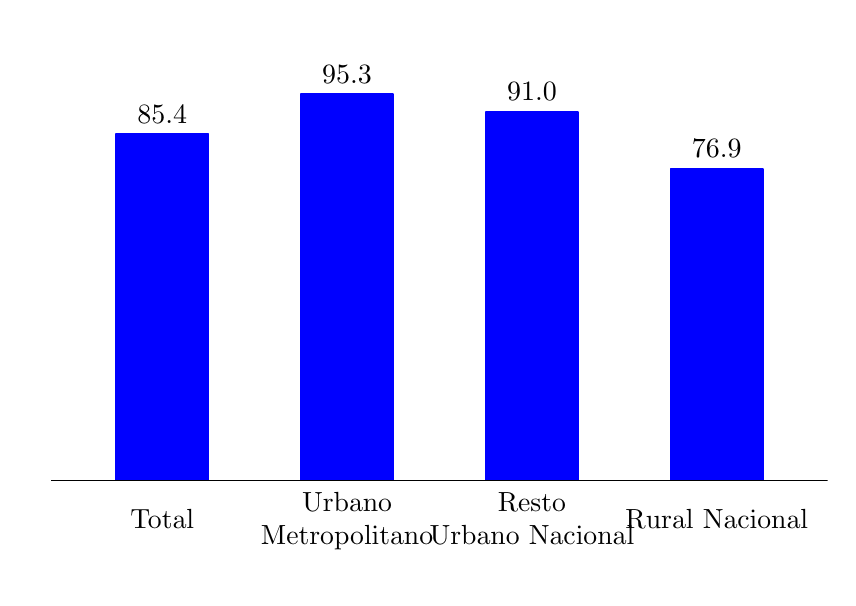
\begin{tikzpicture}[x=1pt,y=1pt]  % Created by tikzDevice version 0.9 on 2015-12-11 10:47:36
% !TEX encoding = UTF-8 Unicode
\definecolor{fillColor}{RGB}{255,255,255}
\path[use as bounding box,fill=fillColor,fill opacity=0.00] (0,0) rectangle (289.08,198.74);
\begin{scope}
\path[clip] (  0.00,  0.00) rectangle (289.08,198.74);

\path[] (  0.00,  0.00) rectangle (289.08,198.74);
\end{scope}
\begin{scope}
\path[clip] (  0.00,  0.00) rectangle (289.08,198.74);

\path[] (  8.54, 28.23) rectangle (289.08,181.67);

\path[] ( 48.61, 28.23) --
	( 48.61,181.67);

\path[] (115.41, 28.23) --
	(115.41,181.67);

\path[] (182.21, 28.23) --
	(182.21,181.67);

\path[] (249.00, 28.23) --
	(249.00,181.67);
\definecolor{drawColor}{RGB}{0,0,255}
\definecolor{fillColor}{RGB}{0,0,255}

\path[draw=drawColor,line width= 0.6pt,line join=round,fill=fillColor] ( 31.91, 35.21) rectangle ( 65.31,160.24);

\path[draw=drawColor,line width= 0.6pt,line join=round,fill=fillColor] ( 98.71, 35.21) rectangle (132.11,174.70);

\path[draw=drawColor,line width= 0.6pt,line join=round,fill=fillColor] (165.51, 35.21) rectangle (198.91,168.34);

\path[draw=drawColor,line width= 0.6pt,line join=round,fill=fillColor] (232.30, 35.21) rectangle (265.70,147.71);
\definecolor{drawColor}{RGB}{0,0,0}

\path[draw=drawColor,line width= 0.1pt,line join=round] (  8.54, 35.21) -- (289.08, 35.21);

\node[text=drawColor,anchor=base,inner sep=0pt, outer sep=0pt, scale=  1.01] at ( 48.61,164.19) {85.4};

\node[text=drawColor,anchor=base,inner sep=0pt, outer sep=0pt, scale=  1.01] at (115.41,178.65) {95.3};

\node[text=drawColor,anchor=base,inner sep=0pt, outer sep=0pt, scale=  1.01] at (182.21,172.29) {91.0};

\node[text=drawColor,anchor=base,inner sep=0pt, outer sep=0pt, scale=  1.01] at (249.00,151.66) {76.9};

\path[] (  8.54, 28.23) rectangle (289.08,181.67);
\end{scope}
\begin{scope}
\path[clip] (  0.00,  0.00) rectangle (289.08,198.74);

\path[] (  8.54, 28.23) --
	(  8.54,181.67);
\end{scope}
\begin{scope}
\path[clip] (  0.00,  0.00) rectangle (289.08,198.74);

\path[] (  8.54, 28.23) --
	(289.08, 28.23);
\end{scope}
\begin{scope}
\path[clip] (  0.00,  0.00) rectangle (289.08,198.74);

\path[] ( 48.61, 23.96) --
	( 48.61, 28.23);

\path[] (115.41, 23.96) --
	(115.41, 28.23);

\path[] (182.21, 23.96) --
	(182.21, 28.23);

\path[] (249.00, 23.96) --
	(249.00, 28.23);
\end{scope}
\begin{scope}
\path[clip] (  0.00,  0.00) rectangle (289.08,198.74);
\definecolor{drawColor}{RGB}{0,0,0}

\node[text=drawColor,anchor=base,inner sep=0pt, outer sep=0pt, scale=  1.00] at ( 48.61, 17.92) {Total};

\node[text=drawColor,anchor=base,inner sep=0pt, outer sep=0pt, scale=  1.00] at (115.41, 23.86) {Urbano };

\node[text=drawColor,anchor=base,inner sep=0pt, outer sep=0pt, scale=  1.00] at (115.41, 11.98) { Metropolitano};

\node[text=drawColor,anchor=base,inner sep=0pt, outer sep=0pt, scale=  1.00] at (182.21, 23.86) {Resto };

\node[text=drawColor,anchor=base,inner sep=0pt, outer sep=0pt, scale=  1.00] at (182.21, 11.98) { Urbano Nacional};

\node[text=drawColor,anchor=base,inner sep=0pt, outer sep=0pt, scale=  1.00] at (249.00, 17.92) {Rural Nacional};
\end{scope}
  \end{tikzpicture} }{Instituto Nacional de Estadística, con datos de ENEI II-2014}